\documentclass[aps,prl,showpacs,twocolumn,amsmath,amssymb,superscriptaddress]{revtex4-2}

\usepackage{tabularx}
\usepackage{bm}
%\usepackage[demo]{graphicx}
\usepackage{graphicx}
\usepackage{tikz}
\usepackage{breqn}

\usepackage{hyperref}
\hypersetup{colorlinks=true,urlcolor= blue,citecolor=blue,linkcolor= blue,bookmarks=true,bookmarksopen=false}

\usepackage{color}

\usepackage{multirow}
\usepackage{dcolumn}
\usepackage{amssymb,amscd,xypic,bm,wasysym}
\usepackage{float}
\usepackage{cleveref}
%\newcolumntype{Y}{>{\centering\arraybackslash}X}

\newcommand{\Red}[1]{\textcolor{red}{#1}}
\usepackage{soul}  % \st    for strike-out
\renewcommand{\vec}[1]{\mathbf{#1}}

\begin{document}

\title{Unveiling quantum Hall effect in spatially inhomogeneous Floquet systems without external magnetic field}
\author{M. Tahir}
\affiliation{Department of Physics, Colorado State University, Fort Collins, CO 80523, USA}
\author{Hua Chen}
\affiliation{Department of Physics, Colorado State University, Fort Collins, CO 80523, USA}
\affiliation{School of Advanced Materials Discovery, Colorado State University, Fort Collins, CO 80523, USA}

\begin{abstract}
Motivated by the recent discovery of Floquet systems, we demonstrate that these produce an unconventional form of the quantized
Landau levels and the corresponding quantum Hall effect without need of an external perpendicular magnetic field. The unconventional quantization in Floquet systems is caused by employing two linearly polarized laser lights in the off-resonant regime with one light being spatially inhomogeneous. This notably distinguishes Landau levels in nonequilibrium Floquet systems from conventional quantum Hall effects observed in equilibrium under the application of strong magnetic field. These results exhibit the fundamental question of realizing quantum Hall effect in nonequilibrium systems and point to a new direction for nano-electronic devices.

We elucidate the origin of the quantized Hall conductance and the Berry phase by using the Floquet theory--adiabatic trajectory of wave packets.
\end{abstract}

\maketitle

\section{Introduction}

The quantum Hall effect (QHE) in conventional two-dimensional electron gas (2DEG) is one of the most remarkable phenomena in condensed matter physics \cite{QHE1}. This effect is indeed associated with a uniform external perpendicular magnetic field, which splits the electron energy spectrum into discrete Landau levels (LLs). Subject to a strong magnetic field, the diagonal (longitudinal) electric conductivity is vanishingly small, while the nondiagonal (Hall) conductivity is quantized. This happens due to the fact that, when the Fermi energy lies in the gap between two LLs, it is referred to as integer QHE as the Hall conductivity takes values of $2(n + 1)e^2/h$ with an integer $n$. Recent experimental realization of graphene has stimulated additional interest to explore QHE in two dimensional systems \cite{QHE2, QHE3, QHE4}. Graphene exhibits unusual quantized Hall conductivity values of $2(2n + 1)e^2/h$ due to application of the magnetic field \cite{QHE4}, which are different from conventional 2DEG.

This significant effect is important to explore in Floquet systems \cite{NHL, AEE} because one may want to observe new phases in an alternative venue that can be experimentally realized \cite{MCR, YHW, HZJ, JWM}. Time periodically modulated Floquet theory has been extensively studied and well established for a large class of systems \cite{JHS,HSA,MGP,MBL,AEE,NGJ}. Therefore, one may employ the high frequency expansions \cite{MBL,AEE,NGJ,SRI,API,TMS,ESM,TKT,ALA} such as the well known Floquet-Magnus expansion \cite{ESM,TKT,ALA,FCA} and Van Vleck expansion \cite{MBL,AEE}. The significant difference is that latter provides an explicit formulas for the time evolution operator starting at initial time $t_{0}=0$ rather than former starting with finite time $t_{0}$ \cite{supp}. In such nonequilibrium systems, a circularly polarized laser light made topology nontrivial in spite of triviality in equilibrium \cite{TKO}. This nontrivial topology is similar to the quantum Anomalous Hall effect proposed by Haldane \cite{Haldane}. Further, optical manipulation of matter is emerging as a promising way of exploring novel phases \cite{AKA, JHM}. This leads to Floquet-Bloch states exhibiting emerging physical properties that are otherwise inaccessible in equilibrium \cite{LST}, i.e., the Floquet Chern insulator \cite{AGG}, Floquet notion of magnetic and other strongly-correlated phases\cite{MSR}, topological classifications, symmetry-breaking concept, and symmetry protected topological phases in nonequilibrium quantum many-body systems \cite{EKM, MSR}. Furthermore, it is important to note that these studies have been demonstrated in the presence of time-periodic homogeneous laser lights. However, the application of spatially inhomogeneous \cite{SWP1, SWP2, SWP3, SWP4, SWP5} laser lights have not been considered so far to best of our knowledge.

In this Letter, it is stirring to unveil that QHE can be observed in Floquet systems without need of uniform magnetic field. We show that two linearly polarized lights are an effective and versatile way of realizing QHE either in graphene-like 2D systems or in conventional 2DEG. Additionally, any one or both lights need to be spatially inhomogeneous. Employing the Floquet theory, we rely on the standard degenerate perturbation formalism and use the Van Vleck expansion \cite{MBL, supp, AEE}. Finally, to obtain the effective Hamiltonian and corresponding bandstructure, we employ the long wavelength limit for spatially inhomogeneous modulation. We believe that our work provides a new platforms for realizing QHE and related novel phases in nonequilibrium systems.

\section{Floquet LLs in Dirac systems}
Dirac electrons can be represented with a generic model Hamiltonian like 2D graphene monolayer,
\begin{equation}\label{eq:HDirac}
	H^D=v_F(\sigma _{x}\Pi _{x}+\sigma _{y}\Pi _{y}),
\end{equation}%
where $\vec{\Pi =p+}e\vec{A^D}$, here $\vec{A^D}$ is the vector
potential, $\vec{p}$ is the momentum operator, $v_F$ is the Fermi
velocity of Dirac fermions, $e$ the absolute value of electron charge,
and $\vec{\sigma}$ the Pauli matrices vector in 2D. We have two linearly polarized laser lights with the electric field components
\begin{equation} \label{eq:Efield}
\vec{E}_{1} =E\cos (\omega t)\hat{x},\vec{E}_{2}=E\sin
(Kx)\sin (2\omega t)\hat{y},
\end{equation}%
where second light is spatially inhomogeneous. It is important to note that second light need to have twice higher frequency than first. This is basic requirement to have LLs spectrum in Dirac systems. Further, one light is propagating along y-axis and polarization is along x-axis, and the other is propagating along x-axis and polarization along y-axis. The $\omega $ is frequency of light with time $t$, $%
K=2\pi /a$ with $a$ being the spatial period of the electric field with
amplitude $E$. This form of the field leads ($\vec{E}=-\frac{\partial \vec{A^D}}{\partial t}$) to the following vector potential $\vec{A^D}$
\begin{equation}\label{eq:Avector}
\vec{A^D}=(-V_y\sin (\omega t), V_x \cos (2\omega t),0),
\end{equation}%
where we have $V_{y}=\frac{ev_FE}{\omega },V_{x}=\frac{ev_FE}{2\omega }\sin(Kx)$. Substituting Eq.~\eqref{eq:Avector} into Eq.~\eqref{eq:HDirac}, we arrive at%
\begin{equation}\label{eq:Htime}
H^D(t)=H_{0}^D- \sigma _{x}V_{y}\sin (\omega t)+\sigma _{y}V_{x}\cos 2(\omega
t),
\end{equation}%
where $H_{0}^D=v_F(\sigma _{x} p_{x}+\sigma_{y} p_{y})$. Because of the time-translation symmetry through $A(t+T)=A(t)$ with $T=2\pi /\omega $, one can apply the Floquet theory \cite{AEE, MBL, supp} and obtain an effective Hamiltonian from Eq.~\eqref{eq:Htime}. After performing the Fourier transform of the time-periodicity, first and second order expansion in $\hbar\omega$ terms leads to the final effective Hamiltonian in Eq.~\eqref{eq:Htime} as
\begin{equation} \label{eq:Heffec}
	H_{\rm eff}^D=H_{0}^D-\frac{V_{y}^{2}v_F\sigma_{y}p_{y}}{\hbar^{2}\omega^{2}}
	-\frac{V_{y}^{2}V_{x}\sigma_{y}}{2\hbar^{2}\omega^{2}}-\frac{v_F\sigma
		_{x}(V_{x}^{2}p_{x}+p_{x}V_{x}^{2})}{8\hbar^{2}\omega^{2}}.
\end{equation}
In Eq. ~\eqref{eq:Heffec}, first order term in $\hbar \omega$ that leads to gap at the Dirac point in usual circularly polarized light experiments \cite{YHW, JWM} is zero here due to inhomogeneous nature of laser lights. This effective Hamiltonian can be simplified in the long wavelength limit to
\begin{equation} \label{eq:HeffB}
H_{\rm eff}^D = v_{F}^{\prime}\sigma_{x}p_{x}+v_F\sigma_{y}(p_{y}-eB^Dx)
\end{equation}%
In obtaining Eq.~\eqref{eq:HeffB}, last term in Eq.~\eqref{eq:Heffec} is second order in space and thus zero in the long wavelength limit for the spatially inhomogeneous modulation. Further, we have $v_{F}^{\prime}=v_F/C,B^D=\frac{V_{y}^{2}E}{4\hbar^{2}\omega^{3}C}K,$ with $C=1-V_{y}^{2}/(\hbar^{2}\omega^{2})$. In accordance with Eqs.~\eqref{eq:Heffec} and ~\eqref{eq:HeffB}, there is least anisotropy in the Dirac spectrum in addition to zero gap. Diagonalizing the Hamiltonian in Eq.~\eqref{eq:HeffB}, we obtained the eigenvalues for Dirac system as%
\begin{equation} \label{eq:DiracEner}
	E_{n}^D=\sqrt{n(v_{F}^{\prime}v_FB^D)2e\hbar},
\end{equation}
which is similar to graphene LLs spectrum in the limit of equal velocities. We can have gapped Dirac spectrum by using uniform circularly polarized laser light as observed in experiments \cite{YHW, JWM} or by using any substrate like hBN. It is also important to note that the effective magnetic field strength obtained for Dirac case in Eq.~\eqref{eq:DiracEner} is directly proportional to third order of the electric field and inversely proportional to the product of spatial period and fifth order of the frequency of the polarized light $\propto (E^3/(a\omega^5))$. This factor of the laser lights can be tuned and thus effective magnetic field can be enhanced in such nonequilibrium situations.

\subsection{Dirac Numerical Approach}

\begin{figure}[h]
  \begin{tikzpicture}
    \node[inner sep=0pt] (figure) at (0,0)
    {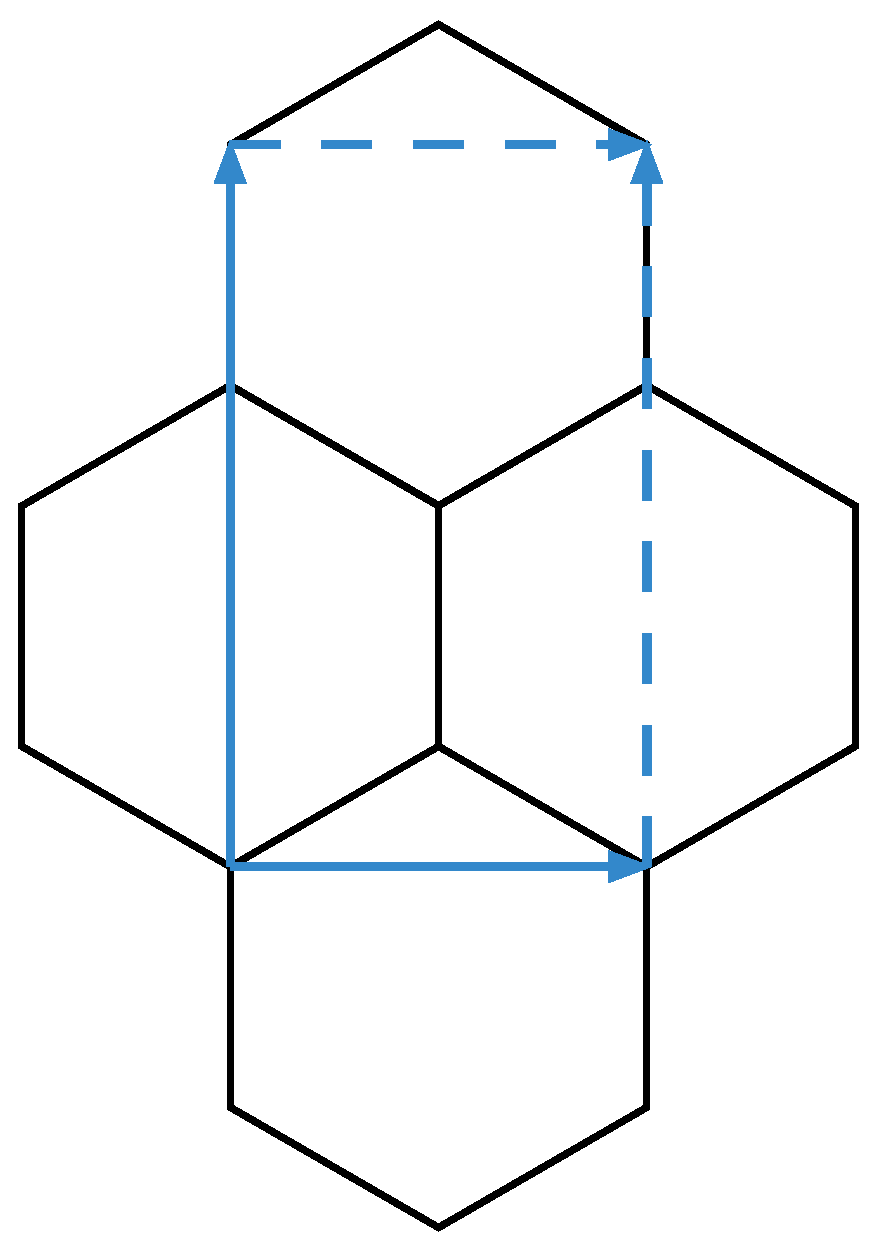
\includegraphics[width=0.25\textwidth]{./figures/dirac-floquet-unit-cell.pdf}};
    \node[inner sep=0pt] (A1) at (-1.3,-1.35) {\small $A_1$};
    \node[inner sep=0pt] (A2) at (-0.3,0.5) {\small $A_2$};
    \node[inner sep=0pt] (B1) at (0.3,-0.5) {\small $B_1$};
    \node[inner sep=0pt] (B2) at (1.35,1.35) {\small $B_2$};
    \node[inner sep=0pt] (a) at (-0.65,-0.75) {\small $a$};
    \node[inner sep=0pt] (a1) at (-1.3,0.0) {\small $\vec{a}_2$};
    \node[inner sep=0pt] (a2) at (0.0,-1.5) {\small $\vec{a}_1$};
  \end{tikzpicture}
  \label{fig:honeycomb}
\end{figure}

We now look beyond perturbation theory.
In doing so we will have to solve the system numerically, which we will describe next.
The incident laser light doesn't allow for translation symmetry along the x-axis for our Dirac honeycomb system.
We consider a simple model using 4 atoms in a unit cell, the lattice vectors are $\vec{a}_1 = \sqrt{3}a\hat{x}$ and $\vec{a}_2 = 3a\hat{y}$, as can be seen in figure \ref{fig:honeycomb}.
Our Hamiltonian takes the following form
\begin{equation}
  H = -\sum_{j'l'\alpha,jl\beta} t^{j'l'\alpha}_{jl\beta} C^{\dagger}_{j'l'\alpha} C_{jl\beta} + h.c.,
\end{equation}
where $t$ is the hopping amplitude, $j,l$ are unit cell index in x and y, and $\alpha,\beta = A_1, A_2, B_1, B_2$.
The vector potential is
\begin{equation}
  \vec{A}(\vec{r},t) = -\dfrac{E}{\omega} \sin{(\omega t)} \hat{x} + \dfrac{E}{2\omega} \sin{(Kx)} \cos{(2\omega t)} \hat{y}.
\end{equation}
To include the vector potential in the tight-binding model we consider a finite system defined by $r_c \geq \max(|x_{i\alpha}|,|y_{i\beta}|)$.
Using a Peierls substitution we can write the hopping term as
\begin{dmath*}
t^{j'l'\alpha}_{jl\beta} = \exp\left[ i \phi_0 \left\{ (x_{j'l'}^{\alpha} - x_{jl}^{\beta}) \sin{\omega t} - \dfrac{1}{2} \sin\left(K \dfrac{x_{j'l'}^{\alpha} + x_{jl}^{\beta}}{2} \right) (y_{j'l'}^{\alpha} - y_{jl}^{\beta}) \cos{2\omega t}  \right\} \right] \\
  = \exp\left[ i X_1 \sin(\omega t) -i X_2 \cos(2\omega t)\right]
\end{dmath*}
where $t=1$ and $\phi_0 = \frac{e E a}{\hbar \omega}$.
One can fourier transform along the y-axis to momentum space to simplify our system to
\begin{equation}
  H = -\sum_{jk} \left[ \Psi^{\dagger}_{jk} H_{j,j} \Psi_{jk} + \Psi^{\dagger}_{j+1,k} H'_{j+1,j,k} \Psi_{jk} + h.c. \right],
\end{equation}
where $\Psi_{jk} = [C_{jkA_1}, C_{jkB_1}, C_{jkA_2}, C_{jkB_2}]^T$. The two matrices are
\[
  H_{j,j} =
  \begin{bmatrix}
    0 & t^{jlA_1}_{jlB_1} & 0 & 0 \\
    t^{jlB_1}_{jlA_1} & 0 & t^{jlB_1}_{jlA_2} & 0 \\
    0 & t^{jlA_2}_{jlB_1} & 0 & t^{jlA_2}_{jlB_2} \\
    0 & 0 & t^{jlB_2}_{jlA_2} & 0
  \end{bmatrix}
\]
and
\[
  H'_{j+1,j,k} =
  \begin{bmatrix}
    0 & t^{j+1,lA_1}_{jlB_1} & 0 & t^{j+1,l+1,A_1}_{jlB_2} e^{i\vec{k}\cdot\vec{a}_2} \\
    0 & 0 & 0 & 0 \\
    0 & 0 & 0 & t^{j+1,lA_2}_{jlB_2} \\
    0 & 0 & 0 & 0
  \end{bmatrix},
\]
where $\vec{k} = k \hat{y}$.
The Hamiltonians dimension is reduced to $N_S \times N_S$, with $N_S = 2r_c+1$.

For Floquet theorem we next consider how to construct the Quasienergy operator $\bar{Q}$.
We first need to calculate the fourier time transform of our Hamiltonian.
Each component of the matrix can be written as the following
\begin{align}
  H_{ab, n} &= \dfrac{1}{T} \int^T_0 H_{ab} e^{-i n \omega t} dt \nonumber \\
  &= \dfrac{1}{2\pi} \int^{2\pi}_0 e^{iX_1\sin(\tau) - iX_2\cos(2\tau) - i n \tau} d\tau.
\end{align}
This integral form is close to a Bessel function but has no elementary solution and we solve it numerically.
The quasienergy matrix $\bar{Q}$ then has matrix elements
\begin{equation}
  \bar{Q}_{m,m+n} = H_n - m \hbar \omega \delta_{n0}
\end{equation}
We choose a cutoff for mode m, $|m| \leq m_c$, where $m_c$ is a positive integer.
This means we will have $N_m = 2 m_c +1$ diagonal blocks, where each block is a $N_S \times N_S$ matrix, $H_n$.

\section{Floquet LLs in 2DEG}
Next, similar to Dirac electrons, we consider the case of Schr\"{o}dinger electrons under the application of two linearly polarized laser lights. The unperturbed Hamiltonian for 2DEG is%
\begin{equation}\label{eq:H2DEG}
H=\frac{\pi_{x}^{2}}{2m^{\ast}}+\frac{\pi_{y}^{2}}{2m^{\ast}},
\end{equation}
where $m^{\ast}$ is the effective mass of electron. By changing the Hamiltonian into a time-dependent form by applying two linearly polarized lights
such that $\vec{\pi\rightarrow p-eA(t)}$. \ Therefore, Eq.~\eqref{eq:H2DEG} is written as%
\begin{equation}\label{eq:H2time}
H(t)=\frac{1}{2m^{\ast}}[p_{x}+eA_{x}(t)]^{2}+\frac{1}{2m^{\ast}}[p_{y}%
+eA_{y}(t)]^{2},
\end{equation}
where the electric field components for two spatially inhomogeneous linearly polarized laser lights are
\begin{equation} \label{eq:E2field}
\vec{E}_{1} =E\cos (\omega t)\hat{x},\vec{E}_{2}^{\prime}=E\cos
(Kx)\sin (\omega t)\hat{y}.
\end{equation}%
It is important to note that second electric field in Eq.~\eqref{eq:E2field} is different from similar field used for Dirac spectrum given in Eq.~\eqref{eq:Efield}. This is due to the fact that Schr\"{o}dinger Hamiltonian is quadratic rather than linear as in case of Dirac electrons. This is basic requirement for the Schr\"{o}dinger electron spectrum to exhibit LLs. The field give in Eq.~\eqref{eq:E2field} lead to the following vector potential $\vec{A}(t)$
\begin{equation}\label{eq:A2vector}
\vec{A}(t)=(-V_1\sin (\omega t), V_2 \cos (\omega t),0),
\end{equation}%
where we have $V_{1}=\frac{eE}{\omega },V_{2}=V_1\cos(Kx)$. Employing the Floquet theory similar to Dirac electrons, we obtain the effective Hamiltonian as%
\begin{equation}\label{eq:H2effec}
	H_{\rm eff}  =H_{0} -\frac{U}{m^{\ast}}\sin (Kx) p_{y} -\frac{U^2}{4m^{\ast}}V_{1}^{2}\cos(2Kx).
\end{equation}
For Landau Level problem, we usually use the Landau gauge with vector potential
like $A=(0,xB,0),B=B\hat{z}$. In the long wavelength limit, Eq.~\eqref{eq:H2effec} can be simplified to
\begin{equation} \label{eq:H2Feffect}
H_{\rm eff}=\frac{p_{x}^{2}}{2m^{\ast}}+\frac{1}{2m^{\ast}}[p_{y}%
+eBx]^{2}-\frac{U^{2}}{4m^{\ast}},
\end{equation}
where $U=\frac{KV_{1}^{2}}{2m^{\ast}\omega}$, and the effective magnetic field
$B=\frac{K^{2}V_{1}^{2}}{em^{\ast}\omega}$. Eq.~\eqref{eq:H2Feffect} is a standard LL problem in the presence of an external perpendicular
magnetic field. Therefore, by diagonalizing the effective Hamiltonian, the corresponding energy eigenvalues are obtained as%
\begin{equation} \label{eq:Energy}
E_{n}=(n+\frac{1}{2})\hbar\omega_{c}-\frac{U^{2}}{4m^{\ast}},
\end{equation}
where $\omega_{c}=\frac{eB}{m^{\ast}}$. We can see from Eq.~\eqref{eq:Energy} that the effective magnetic field is directly proportional to the strength of the electric field (second order) and inversely proportional to the product of second order spatial period and third order of the frequency of the laser lights $\propto (E^2/(a^2\omega^3))$. This factor of the lase lights can be tuned to enhance the strength of the effective magnetic field in nonequilibrium systems.

\section{Discussion and conclusion}

Results can be explained with the help of existing experiments \cite{YHW, JWM} and can provide an estimate for the strength of the effective magnetic field to observe LLs and QHE. Analytical structure of Eq.~(\ref{eq:DiracEner}) and Eq.~(\ref{eq:Energy}) is primarily responsible for the LLs spectrum in both the Dirac and Schr\"{o}dinger systems, respectively.
%Therefore, the effective magnetic field strength can be calculated with the help of parameters realized/used/ implemented in these experimental observations.
Although such results are valid for other 2D materials or Schr\"{o}dinger systems, however, for simplicity, we will consider parameters realized for graphene or topological insulators \cite{YHW, JWM}. In these experiments \cite{YHW, JWM}, the strength of the electric field used is $1 \times 10^7$ V/m to $1 \times 10^8$ V/m and the frequency of the light varies from 120 meV to 191 meV.

In case of Dirac electrons, we calculate the effective magnetic field strength using Eq.~(\ref{eq:DiracEner}). For a fixed value of the spatial period of 120 nm and frequency of laser light $\hbar \omega = 191$ meV, the strength of the effective magnetic field is $\approx$ 10 Tesla for electric field strength of $5 \times 10^7$ V/m \cite{JWM}. Moreover, by reducing the spatial period to 12 nm, we obtain the effective magnetic field $\approx$ 98 Tesla for fixed frequency ($\hbar \omega = 191 $ meV) and electric field ($5 \times 10^7$ V/m). This is due to the fact that effective magnetic field is directly proportional to electric field and inversely proportional to the spatial period of light according to Eq.~(\ref{eq:DiracEner}). Similarly, keeping the spatial period constant and increasing the electric field strength, we can increase the strength of the effective magnetic field for larger frequencies only. However, for the frequency $\hbar \omega = 191$ meV, we can not go beyond $5 \times 10^7$ V/m value of the electric field irrespective of the spatial period. This limitation is due to the factor "C" in Eq.~(\ref{eq:DiracEner}). Further, using lower light frequency ($\hbar \omega = 120$ meV) as realized in topological insulators experiments \cite{YHW}, the critical strength of the electric field is $2 \times 10^7$ V/m beyond which magnetic field will become negative. Additionally, for larger frequency of 220 meV, the maximum value of electric field $7 \times 10^7$ V/m can be used. It is also important and interesting to note that negative values of the effective magnetic field at larger strengths of light's electric field are fruitful. This is because positive or negative values of the effective magnetic field means (see Eq.~(\ref{eq:HeffB})) that magnetic field is applied either from positive z-axis or negative z-axis. \textbf{This estimate of parameters is equally valid for frequency space expansion results (Fig. 1) obtained numerically and degenerate perturbation (Fig. 2) analysis.}

In case of Schr\"{o}dinger electrons in conventional 2DEG systems, the effective magnetic field strength can be obtained using Eq.~(\ref{eq:Energy}). For a fixed value of the spatial period of 100 nm and light frequency of $\hbar \omega = 191$ meV, the strength of the effective magnetic field is 1 Tesla using electric field of $5 \times 10^7$ V/m. Further, by reducing the spatial period to 10 nm and keeping the electric field ($5 \times 10^7$ V/m) and frequency of light ($\hbar \omega = 191 $ meV) fixed, we obtain the effective magnetic field $\approx$ 106 Tesla. This can be understood from Eq.~(\ref{eq:Energy}). In contrast to Dirac case, by increasing the strength of electric field of light, we can increase the strength of the effective magnetic field values. For example, for fixed period of 100 nm and frequency ($\hbar \omega = 191 $ meV), the effective magnetic field is 17 Tesla for $2 \times 10^8$ V/m. Next, we see the impact of increasing or decreasing frequency and keeping period (100 nm) and electric field ($5 \times 10^7$ V/m) fixed. For decreasing frequency to 120 meV, we obtain larger effective magnetic field (4.3 Tesla) while increasing frequency leads to smaller effective magnetic field (0.7 Tesla at 220 meV light frequency). \textbf{This estimate of parameters is equally valid for frequency space expansion results (Fig. 1) obtained numerically and degenerate perturbation (Fig. 2) analysis.}

In conclusion, we have shown Floquet LLs and the QHE using two linearly polarized lights for graphene-like 2D and conventional 2DEG systems. While using these laser lights, we  need at least one or both polarized lights to be spatially inhomogeneous. We have presented results using frequency space expansion method, degenerate Floquet perturbation theory, tight binding models and numerical model calculations. All the results are agreed well to show Floquet LLs in experimentally accessible parameters range. Also, it is interesting to note that we are flexible to use different values of the electric field strength, frequency or spatial period of the light to realize QHE and control the strength of the effective magnetic field. Therefore, we believe that Floquet LLs and QHE can be observed in the experiments for moderate strength of the spatially inhomogeneous lights \textbf{as shown in Figs. 1 and 2.} Moreover, we expect the potential to host new nano-electronics in nonequilibrium systems.

\begin{acknowledgments}
MT and HC were supported by the start-up funding of CSU. The authors are grateful to Allan MacDonald, Olivier Pinaud, Qian Niu, and Di Xiao for helpful discussions. We also need to include Nobel Laureate name here.
\end{acknowledgments}

\bibliography{QHErefv1}

\end{document}
